\section{Evaluation}


To assess the performance of the colocating scheduler in comparison to other schedulers, we conducted a series of experiments focusing on overall CPU and memory usage. These metrics are critical for evaluating scheduler efficiency and effectiveness under various loads and conditions.

We designed experiments to simulate a cloud cluster environment with colocated online/online and online/offline workloads across different cluster settings.

\subsection{Cluster Configuration}

We tested various cluster settings and made an interesting finding: Kubernetes itself (including the Host OS) requires nearly 1 CPU core and 2GB of memory for each node. Initially, we started with a 1C2G (1 core, 2GB memory) single-node cluster, but it turned out that Kubernetes couldn't even schedule its essential components!

Due to cost concerns, we settled on a 6C10G single-node cluster for our experiments. All Kubernetes components, Spark Operator, Koorinator, and workloads run on the same node but are separated by different namespaces.

Resource details are shown in Table \ref{tab:initial}.

\begin{table}
	\centering
	\begin{tabular}{c|ccc}
		            & Capacity & Allocatable & Requested \\
		\hline
		CPU (Cores) & 6        & 5.92        & 0.695     \\
		Memory (GB) & 9.38     & 7.26        & 1.05      \\
	\end{tabular}
	\caption{Cluster Usage before any other workloads}
	\label{tab:initial}
\end{table}
The total allocatable CPU  is 5.92 Cores, and allocatable memory is 7.26 GB.

\subsection{Workload Settings}

We set up two sets of experiments to simulate high/low usage applications followed by easy/intense Spark workloads. Details are provided in Tables \ref{tab:conf-app} and \ref{tab:conf-spark}.


\begin{table*}[h]
	\centering
	\begin{tabular}{cccccc}
		No. & Scheduler   & CPU Req. & Mem Req. & CPU Avg. Usage & Mem Avg. Usage \\
		\hline
		1.1   & Default     & 3.7C     & 200MB    & 3C             & 100MB          \\
		1.2   & Koordinator & 3.7C     & 200MB    & 3C             & 100MB          \\
		2.1   & Default     & 3.7C     & 200MB    & 0.2C           & 100MB          \\
		2.2   & Koordinator & 3.7C     & 200MB    & 0.2C           & 100MB
	\end{tabular}
	\caption{Application Workload Configuration}
	\label{tab:conf-app}

\end{table*}

\begin{table*}[h]
	\centering
	\begin{tabular}{cccccc}
		No. & Scheduler   & CPU Req. & Mem Req. & Desire Pod Count (Driver/Executor) & Job Type \\
		\hline
		1.1 & Default     & 1        & 512 MB   & 2 (1/1)                            & SparkPI  \\
		1.2 & Koordinator & 1        & 512 MB   & 2 (1/1)                            & SparkPI  \\
		2.1 & Default     & 1        & 512 MB   & 5 (1/4)                            & SparkTC  \\
		2.2 & Koordinator & 1        & 512 MB   & 5 (1/4)                            & SparkTC
	\end{tabular}
	\caption{Spark Workload Configuration}
	\label{tab:conf-spark}
\end{table*}

\subsection{Result}

In both sets of experiments, the application workload requests almost all the allocatable CPU resources. Kubernetes' default scheduler consistently rejects Spark workloads (as shown in Table \ref{tab:res}). However, when we switch to Koorinator, Spark workloads can be executed successfully, utilizing nearly all potentially reusable resources and increasing overall cluster usage.


Figure \ref{fig:res-1} illustrates the results for the second set of experiments. The flat horizontal dashline represents CPU and memory requests for the application workload, while the curved dashlines represent cluster CPU and memory usage using the default scheduler. The difference between the red horizontal dashline and the curved dashline represents the potentially reusable resources. The solid lines represent cluster usage after switching to Koordinator.

We observed a significant increase in overall cluster usage. Notably, in experiment 2.2, although the Spark application ends successfully, only 2-3 requested executors are scheduled. This limitation is due to the application's headroom, which is nearly 1.2C (35\% * 3.7), preventing more executors from being colocated.

\begin{table}[h]
	\centering
	\begin{tabular}{ccc}
		No. & Scheduler   & Spark Workload Result \\
		\hline
		1.1   & Default     & Rejected              \\
		1.2   & Koordinator & Finished              \\
		2.1   & Default     & Rejected              \\
		2.2   & Koordinator & Finished*
	\end{tabular}
	\caption{Experiments Result}
	\label{tab:res}
\end{table}

\begin{figure}[h]
	\centering
	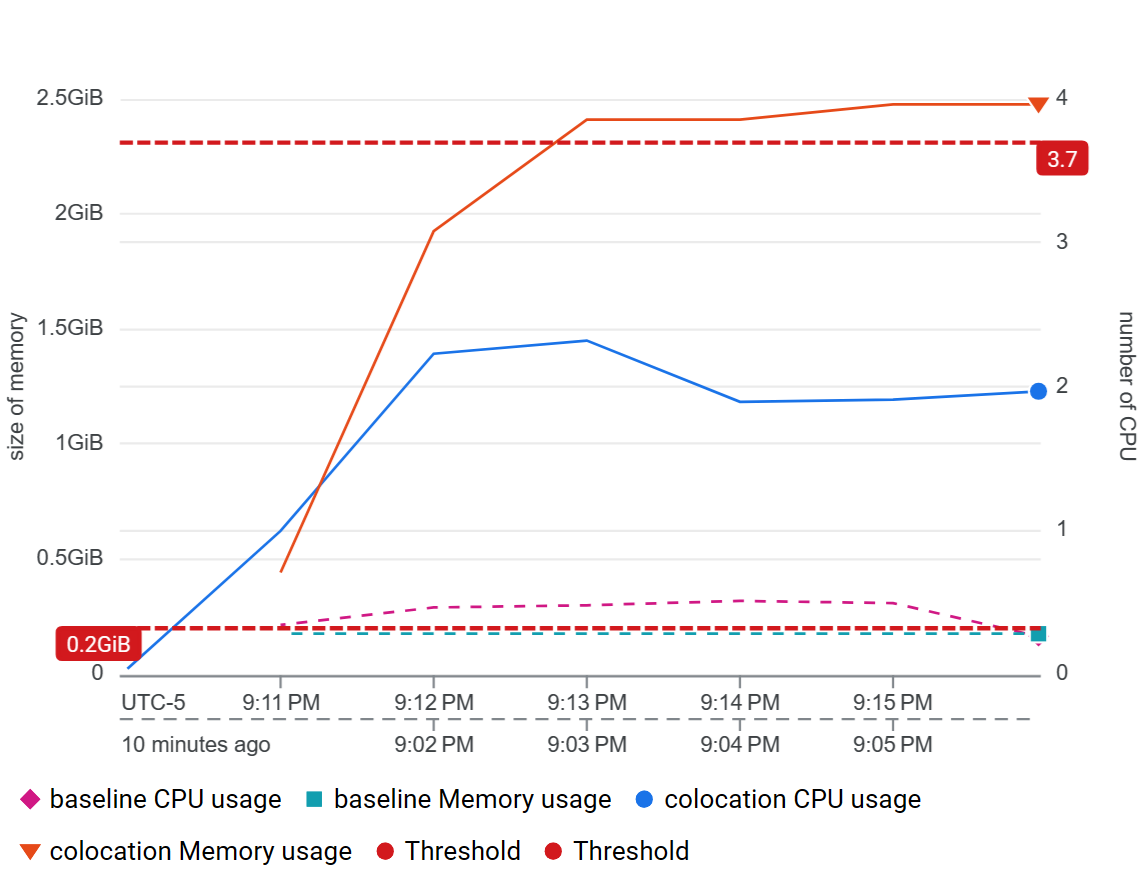
\includegraphics[width=0.5\textwidth]{img-eva-expr1.png}
	\caption{Result for 2nd Set of Experiments}
	\label{fig:res-1}
\end{figure}
